\chapter{\label{chap:problem}O Problema}
A prática de estabelecer a complexidade computacional de jogos -- sejam jogos de
carta, jogos de tabuleiro ou jogos digitais -- ajuda a compreender  porque
humanos consideram interessantes os desafios impostos por estes jogos, além de
indicar para pesquisadores da área os desafios propostos vistos de uma
perspectiva de tarefa de otimização.  Dados os desafios presentes em Spelunky
concluiu-se que, computacionalmente falando, trata-se de um problema, no melhor
dos casos, do conjunto \textit{NP-Hard}\cite{SPELUNKYHARD}. O jogo apresenta uma
série de características -- abordadas em detalhe no capítulo \ref{chap:spelunky}
que influenciam fortemente na dificuldade imposta pelo jogo.

Os níveis trazem grandes dificuldades aos jogadores. Em primeiro lugar, pois o
ambiente em Spelunky é \textbf{contínuo}, \textbf{parcialmente observável},
\textbf{dinâmico}, \textbf{estocástico} e \textbf{sequencial}. Em segundo
lugar, pois são gerados proceduralmente, impossibilitanto a memorização do
mapa.  Contudo, o algoritmo utilizado para gerar os níveis garante que existe
pelo menos um caminho transponível do início ao fim -- mesmo que com inimigos e
armadilhas no caminho --, sem que seja necessário o uso de bombas ou cordas
para ajudar na desobstrução do caminho e deslocamento. Sabe-se, também, que o
personagem sempre entra em um nível pela parte superior do mapa, e que a saída
sempre está localizada na parte inferior do mapa. Um exemplo de mapa gerado
proceduralmente pode ser observado a seguir:

\begin{figure}[htb!]
\centering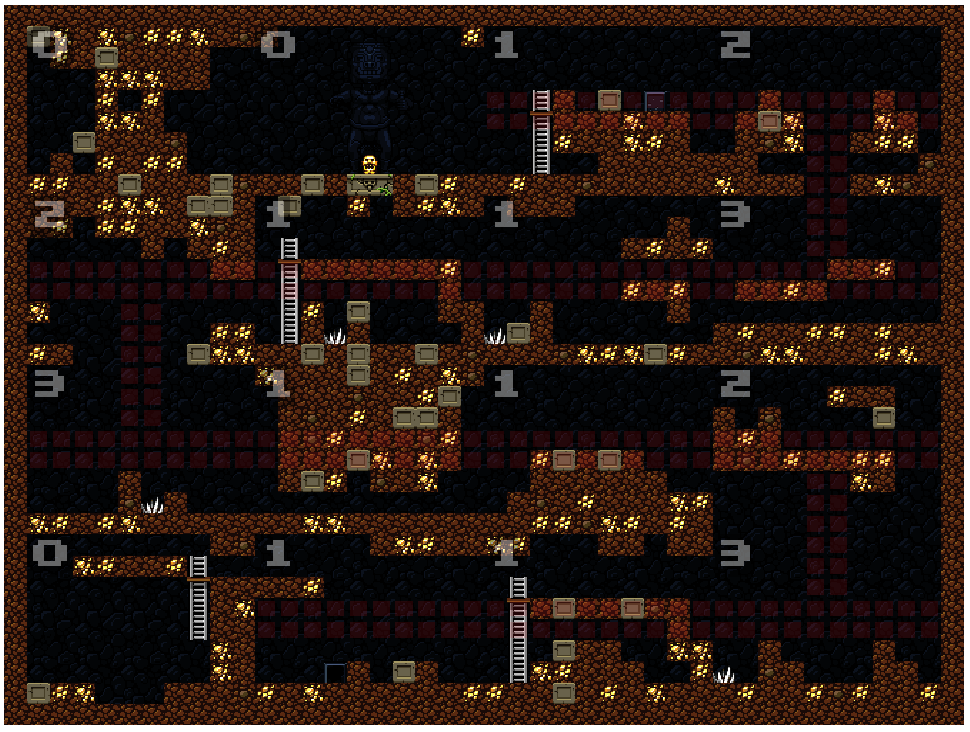
\includegraphics[width=.65\textwidth]{fig/spelunky-level-example.png}
\caption {\label{fig:spelunky-level-example}Exemplo de nível gerado
proceduralmente.} \end{figure}

Em \textit{Spelunky}, os pontos de vida são o recurso mais importante do
jogador, pois quando esgotados, encerra-se a partida. Existem diversos tipos de
inimigos, armadilhas e perigos naturais cujo único objetivo é impedir o
progresso do jogador (detalhados no apêndice \ref{appendix:spelunky-details}).
Somado a isto, depois de 150 segundos em um nível, o jogador será perseguido
incansávelmente por um fantasma que o elimina com apenas um toque, o que impõe
um ''limite`` de tempo que o jogador pode permanecer em um nível.

O jogo permite que o jogador execute um grande número de ações -- e combinações
de ações -- a cada etapa de atualização do jogo. Algumas delas são influenciadas
por itens equipados ou o estado atual do jogador (no ar, pendurado, etc.), o que
significa que a inteligência artificial desenvolvida deve estar preparada pra
lidar com uma gama gigantesca de possibilidades, pois se não houver cautela, a
execução de uma ação pode gerar resultados inesperados. 

Com estes desafios e dificuldades em mente, este trabalho se propõe a
desenvolver \textit{bots} para o jogo \textit{Spelunky}, que terão como
\textbf{objetivo principal} o deslocamento do início ao fim de todos os quatro
níveis de uma das áreas do jogo. Como cada área tem suas peculiaridades -- tais
como monstros e terrenos diferentes --, escolhemos a área das \textbf{minas},
por tratar-se da primeira área do jogo, sendo uma das mais fáceis de se jogar.
Para tal, utilizar-se-á a ferramenta \textit{SpelunkBots} (detalhada no
captítulo \ref{chap:spelunkbots}), que auxilia no desenvolvimento de uma
inteligência artificial para o jogo.
